\documentclass{standalone}
\usepackage{tikz}
\usepackage{ctex,siunitx}
\setCJKmainfont{Noto Serif CJK SC}
\usepackage{tkz-euclide}
\usepackage{amsmath}
\usetikzlibrary{patterns, calc,3d}
\usetikzlibrary{decorations.pathmorphing,decorations.pathreplacing,decorations.shapes}
\begin{document}
\small
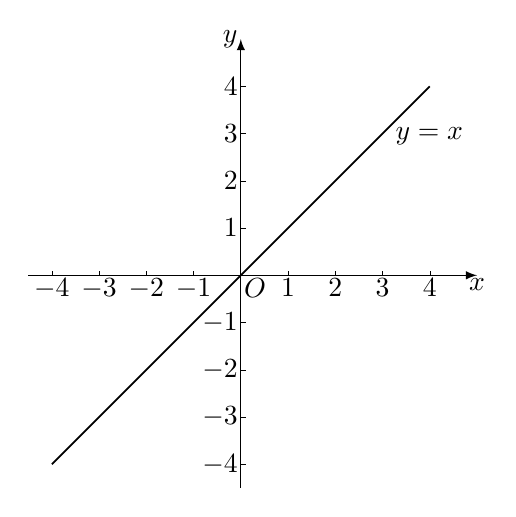
\begin{tikzpicture}[>=latex,scale=0.6,inner sep=1pt]
  \draw[->](-4.5,0)--(5,0)node[below]{$x$};
  \draw[->](0,-4.5)--(0,5)node[left]{$y$};
  \node at (0,0)[below right]{$O$};
  \foreach \x in {-4,-3,...,-1,1,2,...,4}
  {
    \draw[very thin](\x,0)node[below]{$\x$}--++(0,0.1);
    \draw[very thin](0,\x)node[left]{$\x$}--++(0.1,0);
  }
  \draw[semithick](-4,-4)--(4,4)node[pos=0.9,below right]{$y=x$};
\end{tikzpicture}
\end{document}